\documentclass[11pt]{article}
\usepackage{amsfonts,amsmath,latexsym,enumitem,amsthm,amsbsy}
\usepackage{xcolor}
\usepackage{tikz}
\usetikzlibrary{fit,shapes, arrows.meta,bending}
\usetikzlibrary{decorations.pathreplacing}

\begin{document}

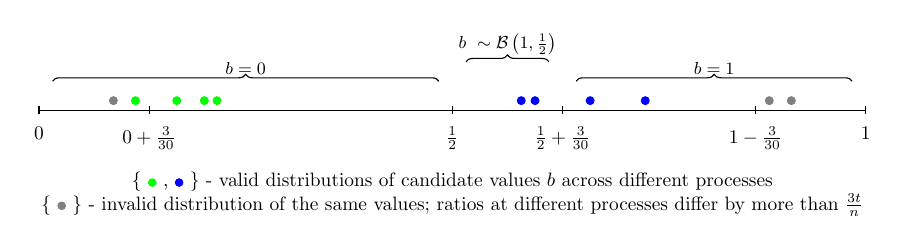
\begin{tikzpicture}[scale=0.7, transform shape]
  % Draw the segment
  \draw (0,0) -- (15,0);

  % Making the inverals
  \foreach \x/\text in {0/0, 2/$0 + \frac{t}{n}$, 7.5/$\frac{1}{2}$, 9.5/$\frac{1}{2} + \frac{t}{n}$, 13/$1 - \frac{t}{n}$, 15/$1$}
    \draw[-](\x, -2pt)--(\x, 2pt);
    
  % Anotating the intervals
  \foreach \x/\text in {0/0, 2/$0 + \frac{3}{30}$, 7.5/$\frac{1}{2}$, 9.5/$\frac{1}{2} + \frac{3}{30}$, 13/$1 - \frac{3}{30}$, 15/$1$}
    \fill (\x,0) circle (0pt) node[below, yshift=-5pt] {\text};

  % Intervals
  \draw[decorate,decoration=brace](0 cm + 7pt, 15pt) -- node[above,font=\small]{$b = 0$} (7.5 cm - 7pt, 15pt);

  \draw[decorate,decoration=brace](7.5 cm + 7pt, 25pt) -- node[above,font=\small]{$b ~\sim \mathcal{B}\left(1, \frac{1}{2}\right)$} (9.5 cm - 7pt, 25pt);
  
  \draw[decorate,decoration=brace](9.5cm + 7pt, 15pt) -- node[above,font=\small]{$b = 1$} (15cm - 7pt, 15pt);


  % Votes skewed towards 1
  \draw[blue, fill=blue] (8.75,5pt) circle (2pt);
  \draw[blue, fill=blue]  (9,5pt) circle (2pt);
  \draw[blue, fill=blue] (10,5pt) circle (2pt);
  \draw[blue, fill=blue] (11,5pt) circle (2pt);
  
  % Votes skewed towards 0
  \draw[green, fill=green] (1.75, 5pt) circle (2pt);
  \draw[green, fill=green] (2.5, 5pt) circle (2pt);
  \draw[green, fill=green] (3, 5pt) circle (2pt);
  \draw[green, fill=green] (3.23, 5pt) circle (2pt);

  %Incorrect votes
  \draw[gray, fill=gray] (1.35, 5pt) circle (2pt);
  \draw[gray, fill=gray] (13.65, 5pt) circle (2pt);
  \draw[gray, fill=gray] (13.25, 5pt) circle (2pt);

  %Legend 
  \node[below, align=center] at (7.5, -1.0) {
    $\{$ \tikz{\draw[green, fill=green] circle (2pt);} ,  \tikz{\draw[blue, fill=blue] circle (2pt);} $\}$ - valid distributions of candidate values $b$ across different processes \\
    
    $\{$ \tikz{\draw[gray, fill=gray] circle (2pt);} $\}$ - invalid distribution of the same values; ratios at different processes differ by more than $\frac{3t}{n}$
  };
  
\end{tikzpicture}

\end{document}